\chapter{User Study}
\label{chap:user}

% More details on the paper.
\chapref{chap:analysis} describes the analyses performed on the data and the resulting conclusion, that only a small portion of indicative tweets can be recovered from the article they link to if viewed as an extractive summarization problem. This conclusion suggests that the next step should be gaining more knowledge about the relation between the tweet and the article in terms of what the tweet does with respect to the article. This information would enable us to figure out if a tweet can actually be generated from summarizing the text in the article. If so, we would then be able to figure out what strategy would be the most appropriate for this task. This task has been explored in this chapter. 

\section{Functions of Tweets}
% Preliminary recommendations on text typology
One aspect of gaining more knowledge would be asking what the \textit{`function'} of the tweet is. If the function of the tweet is known, it might be possible to predict the degree of extractiveness of the tweet with respect to the article. For example, if the function of the tweet is to be an advertisement for a particular product and the text contains the description of the features of the product, then intuitively, the tweet would likely be an extractive summary of the text. On the other hand, if the tweet were an attention grabbing title to merely bring traffic to the text, it would be more likely to be a generic title, than a summary of the actual text. To identify these functions, we first looked at multiple studies aiming to classify functions of tweets. Once functions were isolated and questions to be asked about the tweets finalized, the data was put forth to be classified by human evaluators in a user study.

\subsection{Previous work in classifying function of tweets}
%Having learnt from the tagging attempts earlier, we think that one promising direction is to model the \textit{function}, more explicitly. 
There have been several studies on classifying function of tweets, but in many cases it is described as a more general, high-level intents of the tweets, akin to classifying the topic or genre of the tweet rather than the function. \cite{wang2015mining} use bootstrapping to generate an intent keywords set used in generating an intent graph in a semisupervised manner. They focus on finding tweets with intent and then classifying those. The intent here is defined as a wish or a plan to for some action, such as intent for buying/doing food and drink, travel, career and so on. Classification of intents in this way can directly be used as intents for purchasing and be utilized for advertisements.  \citet{banerjee2012towards} analyze real time data to detect presence of intents in tweets. \citet{gomez2014content} use features from text and stylistics to determine user intentions, which are classified as news report, opinion, publicity and so on. \cite{mohammad2013identifying} use a different take on the intents and use them to study the classification of user intents specifically for tweets related to elections. They study one election and classify tweets as ones that agree or disagree with the candidate, ones that are meant for humour, support and so on. 
%These definitions of intent, while a promising start, will not be sufficient for tweet generation. For this purpose, intent would be the reason the user chose to share the article with that particular text. \cite{sinclair1996preliminary} describe this as 'communicative intent' describing the types as information, discussion, recommendation, recreation, religion and instruction with further subcategories. 


\subsection{Possible functions and questions}

While the definitions described earlier are a promising start, we were looking for a way to model the function in the sense of why the user chose to share the article with the particular text written in the tweet. The closest description found was in \cite{sinclair1996preliminary}, who describe this as `communicative intent' describing the types as information, discussion, recommendation, recreation, religion and instruction with further subcategories. There are also the traditional summary classifications such as evaluative vs descriptive and informative, indicative and critical. 

The first attempt at tagging the dataset were made using the following scheme: a sample set of 100 articles were tagged by two people. The tags used in the preliminary tagging were : `evaluative' vs `descriptive'. `Evaluative' text is a more opinionated text, that is more subjective. This text would be expected to take a certain object or event, analyze it,  and form an opinion about it. `Descriptive' text is non-evaluative, containing for example a narration of an event or an explanation about a certain object or event. A `mixed' category was also added to accommodate some in-between articles. The tagging was done based on the title, article text and tweet. It was observed that this classification was rather subjective, especially between the evaluative/descriptive/mixed tags. Consequently, the Cohen's kappa \citep{kohen1960coefficient} value for correlation turned out to be 0.13, confirming the difficulty of distinguishing these tags. \cite{liu2012survey} give a detailed analysis about classifying evaluative vs descriptive texts, the task is named as subjectivity classification. They point out that it is a bad idea to classify on a sentence level in complex sentences, since a sentence and by extension a text might be factual as well as evaluative, which was the original problem while tagging. These tagging schemes did not yield much success in terms of gleaning information over the entire dataset.

The type of articles being referenced, and the possible reasons these might be shared gave the list of the possible functions. Using these and earlier studies, we enumerated the relevant functions of tweets for our data : promote a product or an article, agree or disagree with an event, or express an opinion about it. Identifying these functions would ideally help provide parameters for generating tweets. These idea behind these functions have been discussed in the following paragraphs. 

If the tweet references a newspaper article, it might be promoting the article, in the sense of attracting people to go further and read the article in more detail. This kind of tweet would try to sensationalize material. It could either tweet the headline of the article directly, or summarize the headline itself further, or simply says something in the likes of `Check this out' or `This is worth a read' and then further categorizes the article with the use of appropriate hashtags indicating the contents of the text.

Example :``Check out this article! \{url\}" or ``Look what this says! \{url\}"

A second option is that the tweet expresses an opinion about something in the article. It could be a positive or a negative comment about the contents of the article or an agreement or disagreement about the events or thoughts and opinions expressed in the article. 

Example : "This is a terrible analysis. {url}" or "Listening to this album on repeat! {url}"

And thirdly, it could be a tweet that singles out a particular piece of information or opinion directly from the article, either to agree with it or to express the importance of the sentence or phrase in the article according to the author of the tweet. It could also be a short summary of the text of the article to either with the aim of inviting readers or just inform readers about the contents of the article.

Example :``Winter approaching, ways to stay safe from flu season: \{url\}"


\section{Running User Study on Amazon Mechanical Turk}

Amazon Mechanical Turk is a crowdsourcing platform that enables researchers to put up huge samples of data along with surveys, quizzes, and simple tasks to be solved by people over the world.

\subsection{Pilot Studies}

 Four pilot studies were conducted on 100 randomly selected tweet and article pairs, using each to improve the questions. For these pilot studies, we tried various combinations of questions and qualifications.
 
 \paragraph{Questions used} All the questions described earlier were experimented with, with the question about emotion giving the highest Fleiss' kappa \citep{geertzen2012inter} between the raters. Since this question was included as a point of interest for future studies, it was dropped going forward with the rest of the studies.
%  The questions used in these studies were the two described above along with another question asking whether the tweet expressed an emotion about the article. It could be a positive or a negative comment about the contents of the article or an agreement or disagreement about the events or thoughts and opinions expressed in the article. 
 
%  Example :``This is a terrible analysis. \{url\}" or ``Listening to this album on repeat! \{url\}"


\paragraph{Qualification settings} Mechanical Turk assigns qualifications to workers based on their skill level in answering questions and their statistics in accepted answers. Workers with superior skills and higher accuracy while answering HITs get the qualification `Masters' which was the qualification used for these pilot studies.

Three separate opinions from the workers were gathered for each tweet and article pair and the agreement calculated using Fleiss' kappa measure  of agreement \citep{geertzen2012inter} between the raters. These pilot studies paved the way towards understanding how the data was being analyzed by outsiders. 
 
 
  % A second option is that the tweet expresses an opinion about something in the article. It could be a positive or a negative comment about the contents of the article or an agreement or disagreement about the events or thoughts and opinions expressed in the article. 

% Example : "This is a terrible analysis. {url}" or "Listening to this album on repeat! {url}"

\subsection{Questions used for the final study}

After the four initial pilot studies, a decision was taken to present the questions separately in two different studies excluding the third question about emotion expressed by tweet. This would guarantee an unbiased opinion about that particular question without any assumptions of either/or questions.

The final questions derived from these functions are shown in \tabref{tab:mturkqs}. A third question of whether the tweet expressed an emotion towards the article, and if so, whether it was a positive or negative emotion was asked too for the purpose of data collection. 

\begin{table}[!htbp]
\centering
\begin{tabular}{|p{0.15\linewidth}|p{0.8\linewidth}|}
\hline
Question 1 & Does the tweet explicitly encourage the reader to visit the link and read the original article? \\ \hline
Question 2 & Does the tweet contain some information from the article, or summarize the article?             \\ \hline
\end{tabular}
\caption{Questions for user study}
\label{tab:mturkqs}
\end{table} 

\subsection{Qualification details}

After playing with the initial setting of `Masters' on the Mechanical Turk, we found the way to obtain the best quality results was to add an additional level of qualification. The qualification test contained three questions from the dataset that had an obvious category for function of tweets. These tests were presented to the workers, and only workers with a 100\% score in these tests were allowed to work on the data. These tests would ensure not only that the worker had a complete understanding of the task at hand, but also be able to come to a correct conclusion in an obvious category situation. A separate pilot with these qualifications and questions structure gave promising results, and the user study was then run on the entire dataset.

\subsection{Running the final study}

\figref{fig:q1} and \figref{fig:q2} show an example of what a HIT (task on Mechanical Turk) for the two questions looked like to the user, respectively.
\begin{figure}[!htbp]
  \centering 
  \subfloat{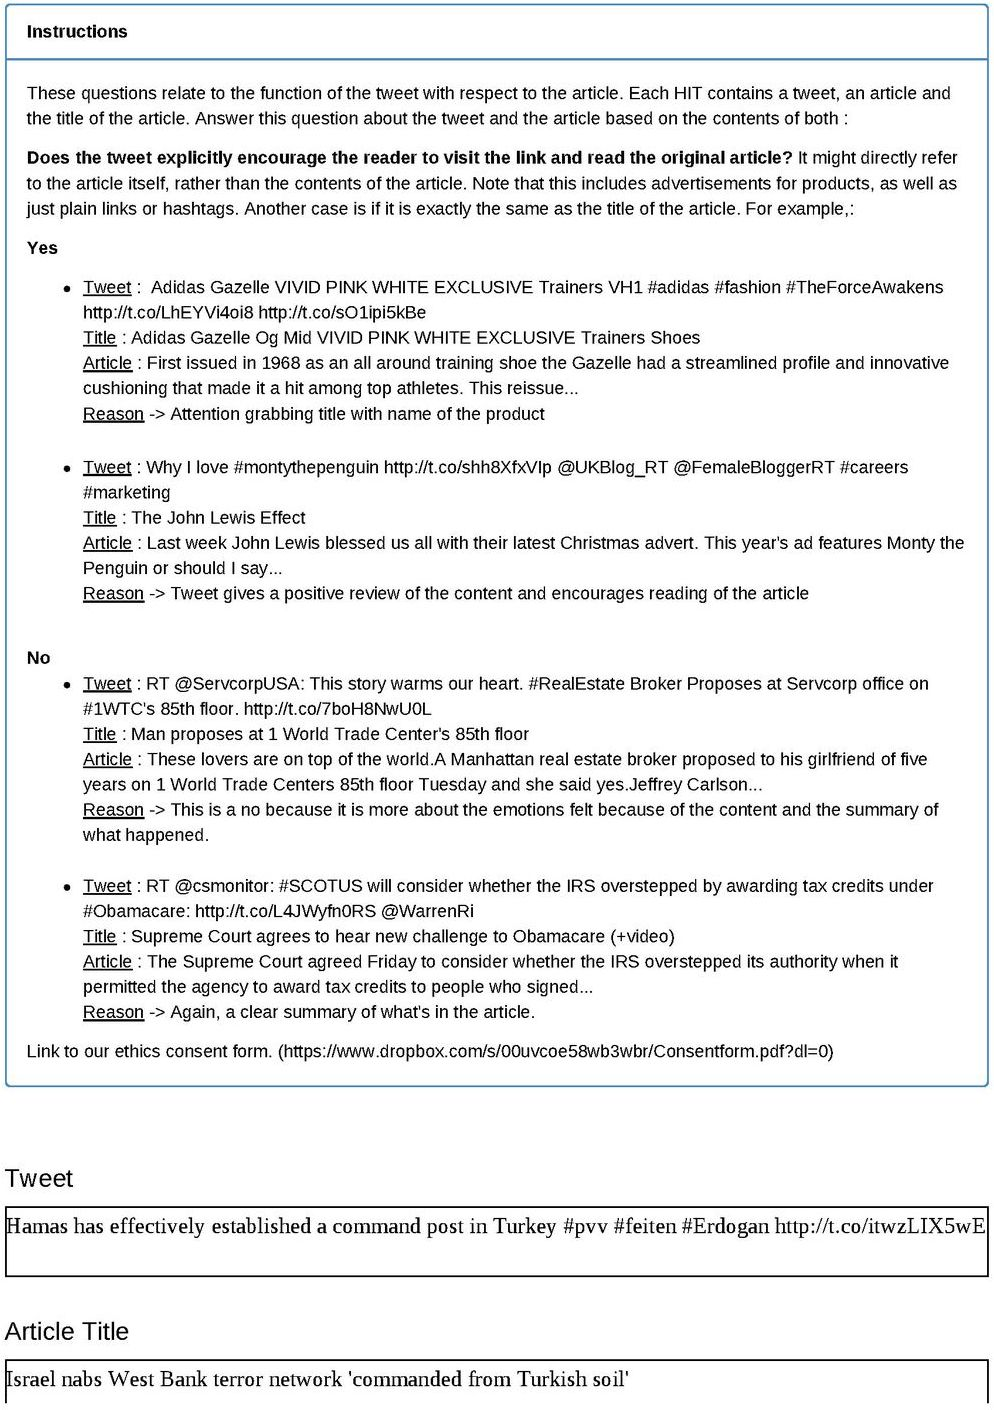
\includegraphics[width=\textwidth, height=21cm]{q11}}
  %\qquad 
  %\subfloat[][b]{q11} 
  \caption[User study question 1 example]{The first question posed for each sample asked to the users.}
  \label{fig:q1}
\end{figure}

\begin{figure}[!htbp]
  \ContinuedFloat 
  \centering 
  \subfloat{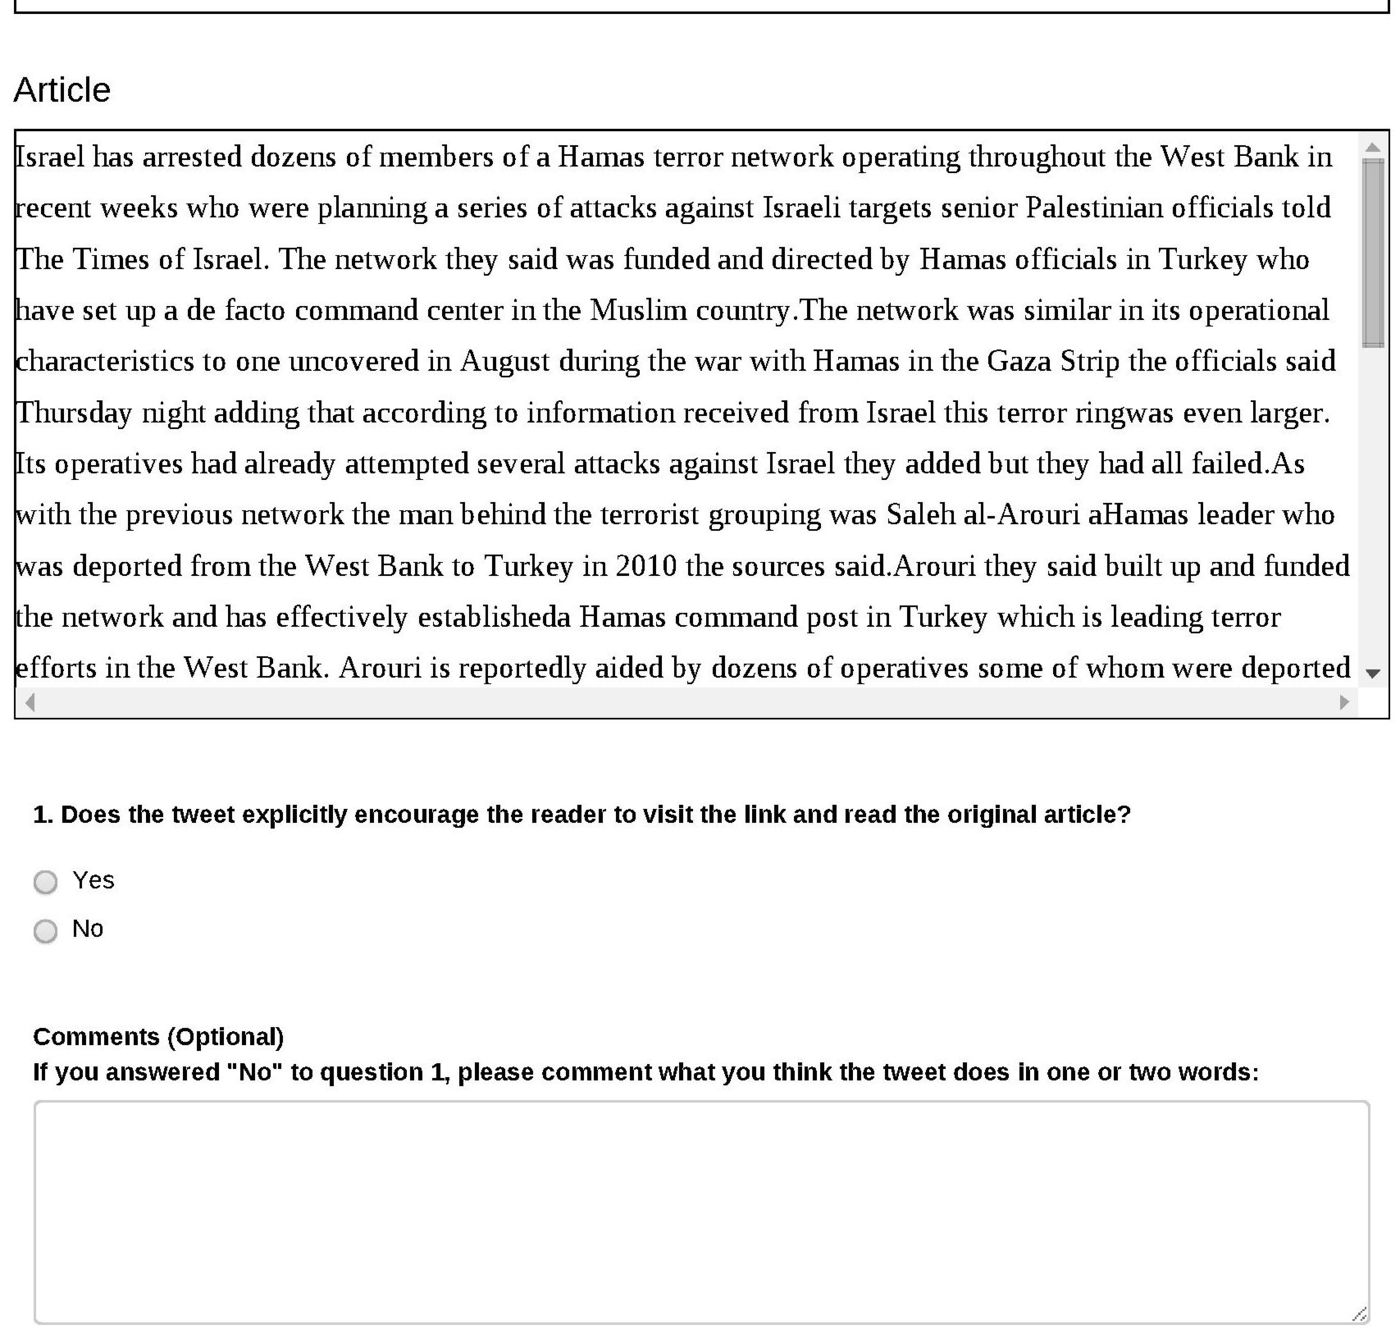
\includegraphics[width=\textwidth, height=13cm]{q12}}% 
  %\qquad 
  %\subfloat[][]{q12} 
  \caption[]{..continued question viewed by users.}
  \label{fig:q12}
\end{figure} 

\begin{figure}[!htbp]
  \centering 
  \subfloat{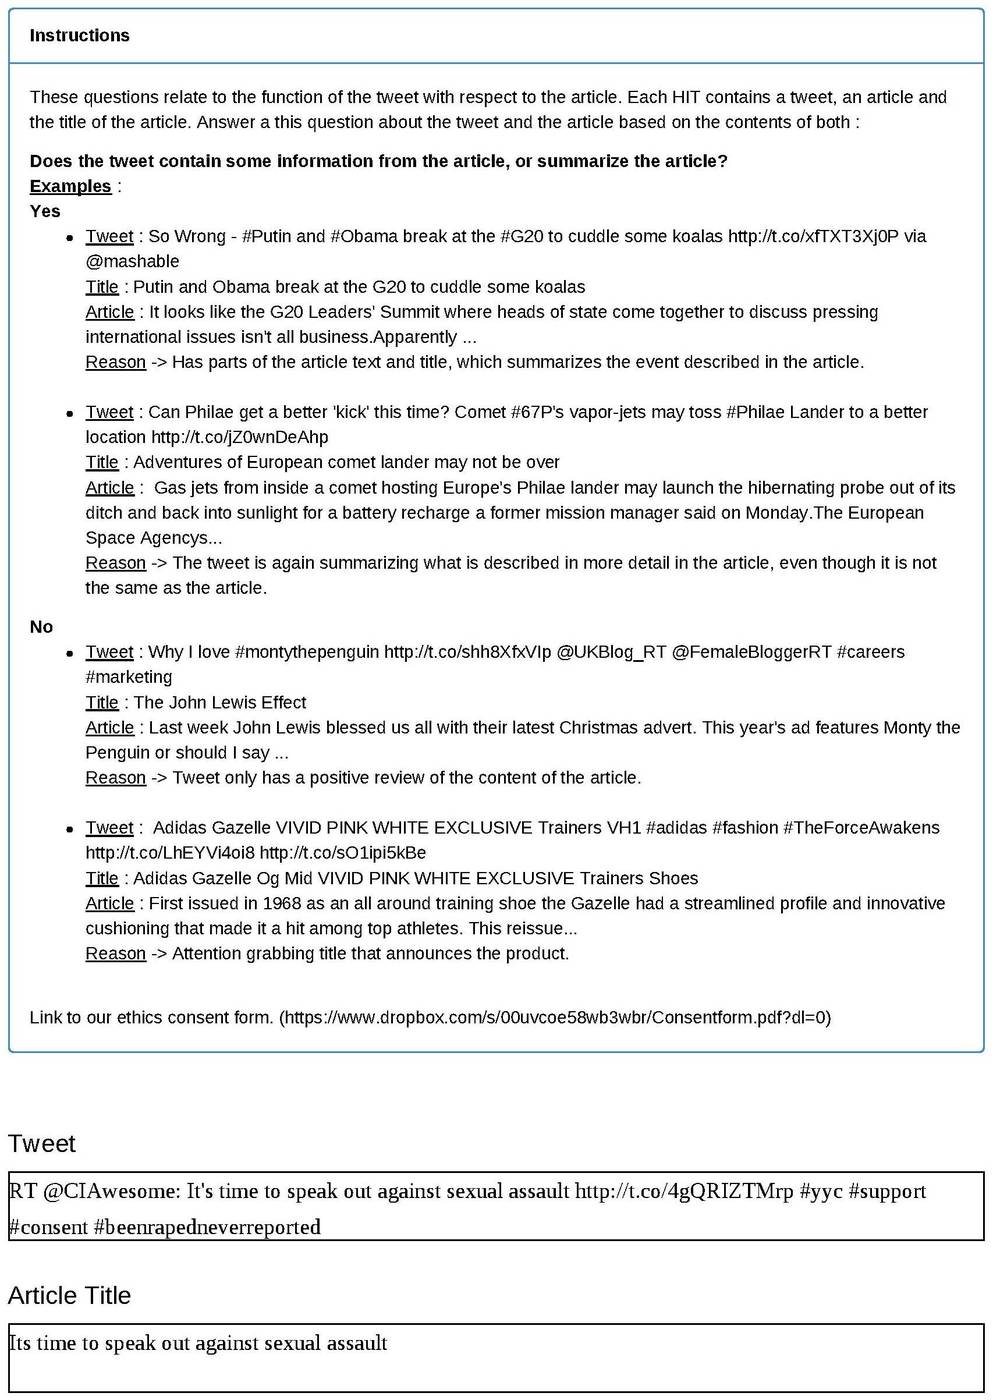
\includegraphics[width=\textwidth, height=21cm]{q21}}
  %\qquad 
  %\subfloat[][b]{q11} 
  \caption[User study question 2 example]{The second question asked for each sample.}
  \label{fig:q2}
\end{figure}

\begin{figure}[!htbp]
  \ContinuedFloat 
  \centering 
  \subfloat{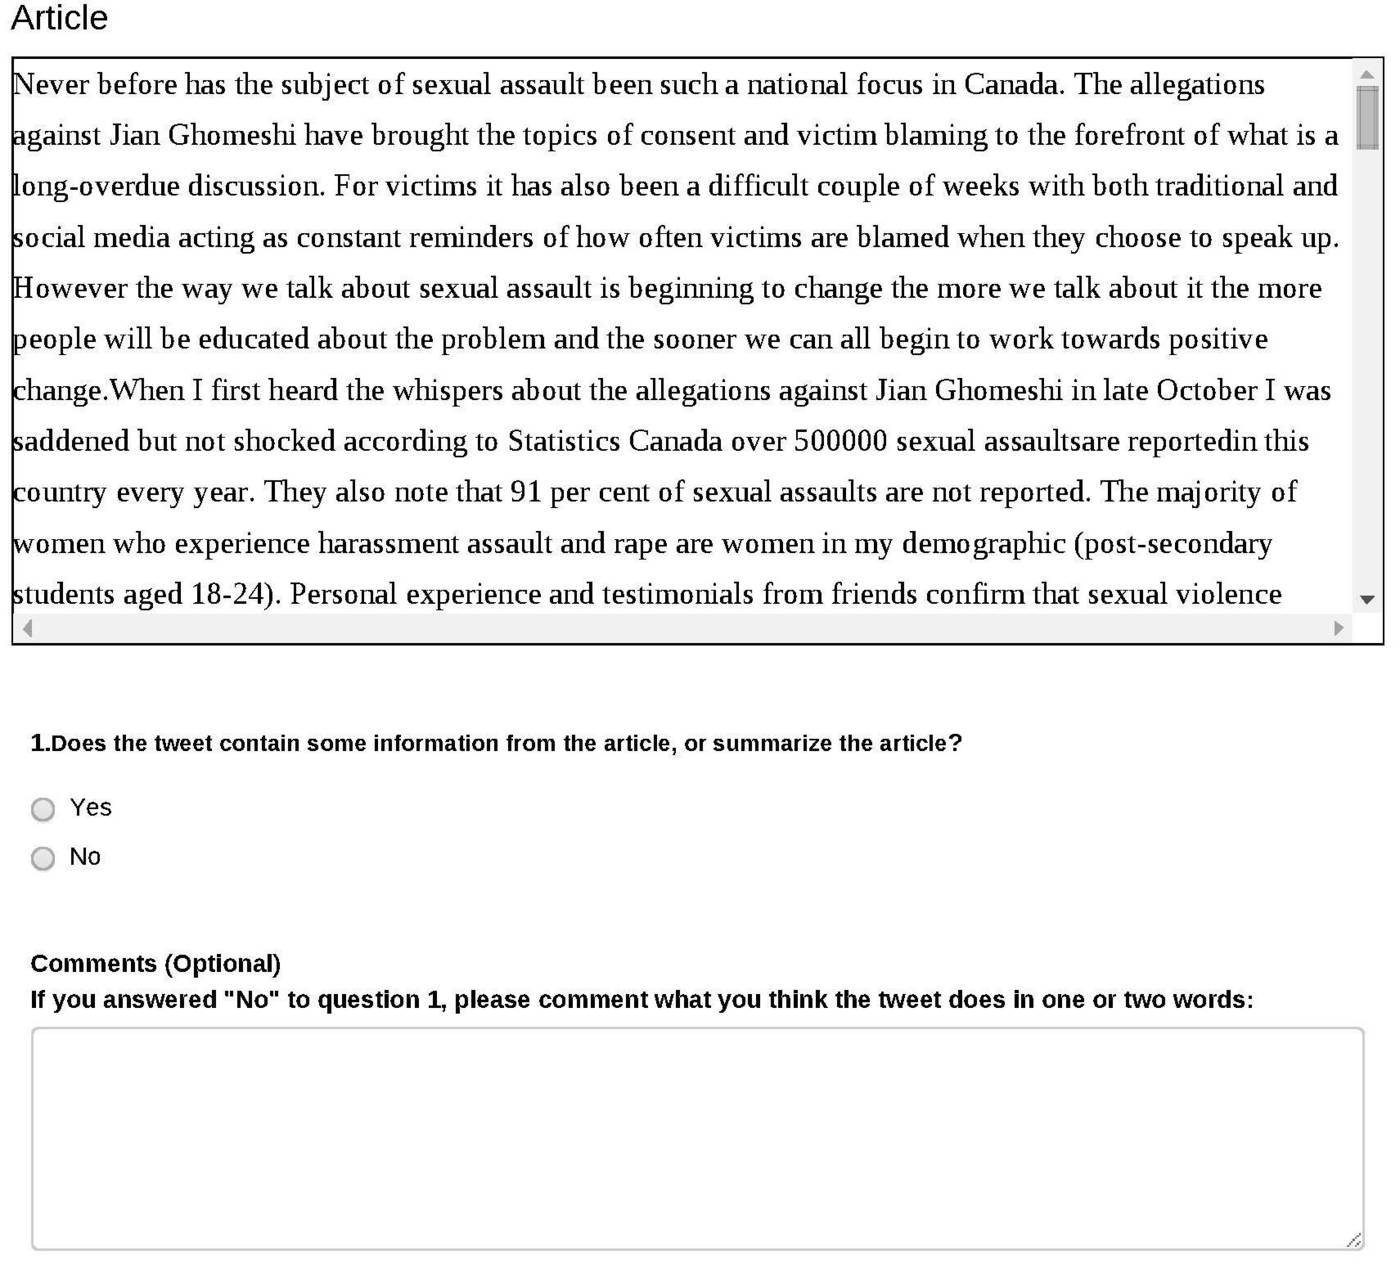
\includegraphics[width=\textwidth, height=13cm]{q22}}% 
  %\qquad 
  %\subfloat[][]{q12} 
  \caption[]{..continued question viewed by users.}
  \label{fig:q22}
\end{figure} 

% * analysis of results from MTurk
%finally separated user studies, 4 pilots
%qualification tests
%mechanical turk CLI
%add forms 
% results can be added later

\subsection{Results and Analysis for User Study}

% \begin{figure}[!htbp]
% \centering
% 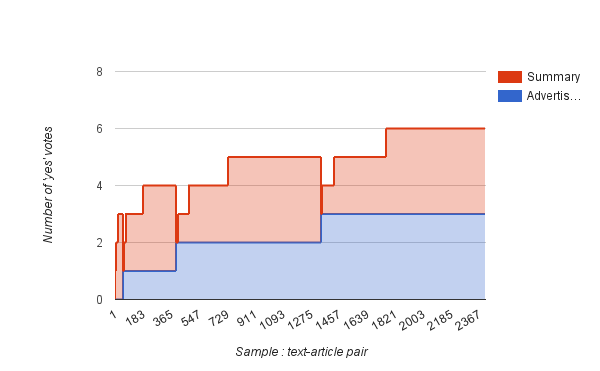
\includegraphics[width=0.9\textwidth, height=9cm]{results}
% \caption[Results from user study]{Visualization for tags from human evaluators}
% \label{fig:res}
% \end{figure}

% The results obtained from the final study are shown in \figref{fig:res}. The bottom line shows the number of 'yes' votes per article and tweet for the first question, whether the tweet was a promotion of the article. The red line on top of it signifies the number of 'yes' votes for the second question, whether the tweet was a summary of the article. 

The total number of `yes' votes for each of the questions are shown in \tabref{tab:yeses}. \tabref{tab:exq1no}, \tabref{tab:exq1yes}, \tabref{tab:exq2no} and \tabref{tab:exq2yes} all show examples where for one of each question, all three workers agreed to a tweet being or not being an advertisement or a summary. The Fleiss' kappa for the first study, showing the indicativeness of the tweet was 0.147 and the kappa for the second study, showing the informativeness of the tweet, was 0.208.

\begin{table}[!htbp]
\centering
\caption{Analysis of user study results}
\label{tab:yeses}
\begin{tabular}{|l|l|l|l|l|}
\hline
Questions     & 0 votes & 1 vote & 2 votes & 3 votes \\ \hline
Advertisement & 53    & 340    & 942     &  1068  \\ \hline
Summary       & 29     & 176    & 703     & 1495    \\ \hline
\end{tabular}
\end{table}


\begin{table}[!htbp]
\centering
\begin{tabular}{|p{0.1\linewidth}|p{0.8\linewidth}|}
\hline
Tweet &   RT @WSJ: In \#CometLanding Philae probe bounced and settled in area that could hinder its research. http://t.co/6lfg3p9XG1 http://t.co/A6fi  \\ \hline
Title &   Rosetta Mission Probe Landed on Comet in Shadow of Cliff	                                                                                 \\ \hline
Text  &  The historic Philae comet probe hit its target but then unexpectedly bounced twice settling in the shadow of a cliff that could hinder its research new images sent back Thursday showed.Philae is designed to run a suite...                                                                                         \\ \hline
\end{tabular}
\captionof{table}{Example where all three workers said it was not an advertisement.}
\label{tab:exq1no}
\end{table}


\begin{table}[!htbp]
\centering
\begin{tabular}{|p{0.1\linewidth}|p{0.8\linewidth}|}
\hline
Tweet & \#GalaxyNote3 \#Lollipop - SamMobile has been teasing us with a number of unfinished builds for a few http://t.co/A0IKYsk4g3 \#Samsung \\ \hline
Title &   Samsung GALAXY Note 3's Android Lollipop Update Surfaces                                                                                 \\ \hline
Text  &  SamMobile has been teasing us with a number of unfinished builds for a few months now. This indicates...                                                                                         \\ \hline
\end{tabular}
\captionof{table}{Example where all three workers said the tweet was an advertisement for article.}
\label{tab:exq1yes}
\end{table}


\begin{table}[!htbp]
\centering
\begin{tabular}{|p{0.1\linewidth}|p{0.8\linewidth}|}
\hline
Tweet & "RT @jakbarali: So my partner Gillian Hnatiw and I had something to say about \#VAW \#LoriDouglas and \#Ghomeshi. http://t.co/6X2zMtCAM0 \\ \hline
Title & "Victim-blaming couched as legitimate judicial inquiry" \\ \hline
Text  & Ghomeshi himself broke the first wave of the story when he took to Facebook to decry the CBCs decision to terminate him... \\ \hline
\end{tabular}
\captionof{table}{Example where all three raters said tweet was not a summary.}
\label{tab:exq2no}
\end{table}

\begin{table}[!htbp]
\centering
\begin{tabular}{|p{0.1\linewidth}|p{0.8\linewidth}|}
\hline
Tweet & RT @PopCulturPriest: Doing a story on California's lottery for @americmag I discovered \#JohnOliver's story had some troubling errors: http \\ \hline
Title & Blowing The Dismount: Last Week Tonight Fudges Its Lottery Story \\ \hline
Text  & Sunday night on the season finale of HBOs new news show Last Week Tonight anchor John Oliver spent half the show... \\ \hline
\end{tabular}
\captionof{table}{Example where all three raters agreed the tweet was a summary.}
\label{tab:exq2yes}
\end{table}

We then analyzed the tags obtained from the study with the analyses results we obtained in \chapref{chap:analysis}. The results for the Mann Whitney U test \citep{mann1947test,wilcoxon1947probability} with different parameters considered are shown. \tabref{tab:unicorr1} and \tabref{tab:unicorr2} show the test results for unigram match percentages, \tabref{tab:bicorr1} and \tabref{tab:bicorr2} for bigram match percentages, and \tabref{tab:lcscorr1} and \tabref{tab:lcscorr2} for longest common subsequence match percentages. Each of these are for the two separate studies respectively.  The test was first done while considering zero `yes' votes as one group and three `yes' votes as another group. The test was also done considering zero or  one `yes' votes out of three in one group and two or three `yes' votes out of three in the other group. For each of these studies for each sample set configuration, the U statistic and the p value are shown. The final two columns in both tables show the mean values of values in each of the groups used in the test. 
%The failure to reject the null hypothesis suggests that no definite distinction can be made between the degree of extraction for tweets that are advertisements for articles or summaries of articles.

\begin{table}[!htbp]
\caption{Mann Whitney U test results for indicativeness: Unigram Match}
\centering
\label{tab:unicorr1}
\begin{tabular}{|p{0.29\textwidth}|p{0.1\textwidth}|p{0.1\textwidth}|p{0.09\textwidth}|p{0.09\textwidth}|p{0.09\textwidth}|p{0.09\textwidth}|}
\hline
Groups considered    & U statistic & p value & Mean of values for Group 1 & Number of samples in Group 1 & Mean of values for Group 2 & Number of samples in Group 2\\ \hline
Group 1: 0 `yes' votes \newline Group 2: 3 `yes' votes &  28104  &  0.931413  &  27.44  & 53 & 28.21 &   1068  \\ \hline
Group 1: 0 or 1 `yes' votes \newline Group 2: 2 or 3 `yes' votes &   406355.5  & 0.365219 & 30.65  & 393 & 29.23 & 2010 \\ \hline
\end{tabular}
\end{table}

\begin{table}[!htbp]
\caption{Mann Whitney U test results for informativeness: Unigram Match}
\centering
\label{tab:unicorr2}
\begin{tabular}{|p{0.29\textwidth}|p{0.1\textwidth}|p{0.1\textwidth}|p{0.09\textwidth}|p{0.09\textwidth}|p{0.09\textwidth}|p{0.09\textwidth}|}
\hline
Groups considered    & U statistic & p value & Mean of values for Group 1 & Number of samples in Group 1 & Mean of values for Group 2 & Number of samples in Group 2\\ \hline
Group 1: 0 `yes' votes \newline Group 2: 3 `yes' votes & 12211 & 0.000055  & 16.69 & 29 & 31.07 & 1495  \\ \hline
Group 1: 0 or 1 `yes' votes \newline Group 2: 2 or 3 `yes' votes & 193411 & 0.000791 & 25.08 & 205 & 29.87 & 2198 \\ \hline
\end{tabular}
\end{table}

\begin{table}[!htbp]
\caption{Mann Whitney U test results for indicativeness: Bigram Match}
\centering
\label{tab:bicorr1}
\begin{tabular}{|p{0.29\textwidth}|p{0.1\textwidth}|p{0.1\textwidth}|p{0.09\textwidth}|p{0.09\textwidth}|p{0.09\textwidth}|p{0.09\textwidth}|}
\hline
Groups considered    & U statistic & p value & Mean of values for Group 1 & Number of samples in Group 1 & Mean of values for Group 2 & Number of samples in Group 2\\ \hline
Group 1: 0 `yes' votes \newline Group 2: 3 `yes' votes & 27871 & 0.851388 & 8.31 & 53 & 9.21 & 1068  \\ \hline
Group 1: 0 or 1 `yes' votes \newline Group 2: 2 or 3 `yes' votes& 406313 & 0.378553 & 12.19 & 393 & 10.29 & 2009 \\ \hline
\end{tabular}
\end{table}

\begin{table}[!htbp]
\caption{Mann Whitney U test results for informativeness: Bigram Match}
\centering
\label{tab:bicorr2}
\begin{tabular}{|p{0.29\textwidth}|p{0.1\textwidth}|p{0.1\textwidth}|p{0.09\textwidth}|p{0.09\textwidth}|p{0.09\textwidth}|p{0.09\textwidth}|}
\hline
Groups considered    & U statistic & p value & Mean of values for Group 1 & Number of samples in Group 1 & Mean of values for Group 2 & Number of samples in Group 2\\ \hline
Group 1: 0 `yes' votes \newline Group 2: 3 `yes' votes & 15006 & 0.004541 & 3.88 & 29 & 11.46 & 1494  \\ \hline
Group 1: 0 or 1 `yes' votes \newline Group 2: 2 or 3 `yes' votes & 201755.5 & 0.013592 & 8.07 & 205 & 10.84 & 2197 \\ \hline
\end{tabular}
\end{table}



\begin{table}[!htbp]
\caption{Mann Whitney U test results for indicativeness: Longest Common Subsequence}
\centering
\label{tab:lcscorr1}
\begin{tabular}{|p{0.29\textwidth}|p{0.1\textwidth}|p{0.1\textwidth}|p{0.09\textwidth}|p{0.09\textwidth}|p{0.09\textwidth}|p{0.09\textwidth}|}
\hline
Groups considered    & U statistic & p value & Mean of values for Group 1 & Number of samples in Group 1 & Mean of values for Group 2 & Number of samples in Group 2\\ \hline
Group 1: 0 `yes' votes \newline Group 2: 3 `yes' votes &  26440.5  &  0.418424  &  42.16  & 53 &  44.24 &   1068  \\ \hline
Group 1: 0 or 1 `yes' votes \newline Group 2: 2 or 3 `yes' votes  &  392910     & 0.870236 &  44.66  & 393 & 44.69 & 2010 \\ \hline
\end{tabular}
\end{table}

\begin{table}[!htbp]
\centering
\caption{Mann Whitney U test results for informativeness: Longest Common Subsequence}
\label{tab:lcscorr2}
% \setlength\extrarowheight{5pt}
\begin{tabular}{|p{0.29\textwidth}|p{0.1\textwidth}|p{0.1\textwidth}|p{0.09\textwidth}|p{0.09\textwidth}|p{0.09\textwidth}|p{0.09\textwidth}|}
\hline
Groups considered    & U statistic & p value & Mean of values for Group 1 & Number of samples in Group 1 & Mean of values for Group 2 & Number of samples in Group 2\\ \hline
Group 1: 0 `yes' votes \newline Group 2: 3 `yes' votes & 18466   & 0.171255 & 38.4 & 29 & 44.47  & 1495 \\ \hline
Group 1: 0 or 1 `yes' votes \newline Group 2: 2 or 3 `yes' votes & 217196.5      &  0.393999    & 43.16    & 205 & 44.83   &  2198\\ \hline
\end{tabular}
\end{table}

The p-values for \tabref{tab:unicorr1}, \tabref{tab:bicorr1} and \tabref{tab:lcscorr1} show non-significant results for both sets of groups for the first question, the indicativesness of the tweet. The U statistic for each case is very high and the results show a $p>0.5$. We thus fail to reject the null hypothesis, that the two sets were pulled from the same distribution. For all these cases, the means of the two groups are very close to the means for the respective analyis, and to each other. Mean for Unigram match is 29.53\%, mean for bigram match is 10.73\% and the mean for LCS match is 44.6\% as seen in \chapref{chap:analysis}. 
%The U statistic for each case is very high and the results show a $p>0.5$. We thus fail to reject the null hypothesis, that the two sets were pulled from the same distribution. The means of the LCS values, indicating the extractiveness of the tweet, are very close to each other. 

The p-values for unigram and bigram match for the second question, indicating the informativeness of the summary, shown in \tabref{tab:unicorr2} and \tabref{tab:bicorr2} are both significant, with $p<0.5$, especially so for the first arrangement of groups where group 1 is zero `yes' votes and group 2 is three `yes' votes. Based on the result of the p-values, we can conclude that these samples are drawn from different populations. If we look at the means of the values in each case, they are sufficiently different, with the mean of the first group being significantly smaller the mean of the values in the second group. \tabref{tab:lcscorr2} also shows a slight difference in the study that asked for the informativeness of the tweet in the zero vs three `yes' votes out of three were considered as the sample set configuration. The U-statistic and p-value are both the least in this case, for longest common subsequence results. However, no significant result can be drawn from this since p-value is still quite high. It is possible that the non-significant result can be explained by the fact that the LCS is a lot more flexible for accommodating words from the overall article, and thus while the means of the two groups show difference in the right direction, the p-value is still high to conclude anything significant. 


The results for the questions whether the tweet has an emotion about the article or not are also included. The Fleiss' kappa for agreement was 0.174. The emotion described here is a positive or negative about the text in the article, not about the subject of the article. These were included in the dataset, but were 
 

\subsection{Conclusions from the User Study}

The significant results from \tabref{tab:unicorr2} and \tabref{tab:bicorr2} confirm that when the tweet is not informative, extractiveness is a wrong direction to pursue. However, we do have inconclusive evidence about whether or not extractiveness of the summary(tweet) overlaps with indicativeness the tweets. Further studies would be required to come to a conclusion about this type of summary classification based on function, and how it interacts with extractiveness of the summary. 

The study shows a promising direction for further studies in function of tweets. In fact, an important result of this section is the generation of a human-tagged dataset of tweet and article pairs, based on the indicativeness and informativeness of the tweets, as well as tagged with emotion of the tweet with respect to the article text. 

The question about whether a tweet summarizes the content of the article gave mostly positive answers, suggesting that according to the workers, if the tweet contained a link to article, it was an indicative summary most of the times. However, according to the extractiveness calculated earlier in \chapref{chap:analysis}, the tweets were not extracted from the articles to a large extent. With the results from the user study performed in this chapter, we can see that when the tweet is used informatively, extractive methods have a higher bound that is still low, similar to what was obtained earlier. This reinforces the earlier conclusion of a need for a more sophisticated tool that summarizes the contents of the article for tweet generation.

% The question about whether a tweet summarizes the content of the article gave mostly postive answers, and the correlation with extractiveness shows that is the tweet is used informatively, then extractive methods give us a higher bound which still not helpful for generating tweets. This reinforces the earlier assumption that tweet generation must be done using a more sophisticated tool that summarizes the contents of the article.

%http://www.graphpad.com/guides/prism/6/statistics/index.htm?how_the_mann-whitney_test_works.htm

